\documentclass{article}

\usepackage{extramarks}

\usepackage{amsmath}
\usepackage{amsthm}
\usepackage{amssymb}
\usepackage{amsfonts}
\usepackage{caption}
\usepackage{subcaption}
\usepackage{listings}

\usepackage{hyperref}

\usepackage{tikz}

\usepackage{algorithm}
\usepackage{algorithmic}
\usepackage[shortlabels]{enumitem}

\usepackage{float,graphicx}

\usepackage{pgfplots}

\usepackage{adjustbox}


\usepackage{array}
\usepackage{pgfgantt}

\usepackage[utf8]{inputenc}

\usepackage{fancyhdr}
\usepackage{fancybox}



\topmargin=-0.45in
\evensidemargin=0in
\oddsidemargin=0in
\textwidth=6.5in
\textheight=9.0in
\headsep=0.25in

% Listings' Styles

\definecolor{codegreen}{rgb}{0,0.6,0}
\definecolor{codegray}{rgb}{0.5,0.5,0.5}
\definecolor{codepurple}{rgb}{0.58,0,0.82}
\definecolor{backcolour}{rgb}{0.96,0.96,0.96}


\lstdefinestyle{python}{
    backgroundcolor=\color{backcolour},
    commentstyle=\color{codegreen},
    keywordstyle=\color{magenta},
    numberstyle=\tiny\color{codegray},
    stringstyle=\color{codepurple},
    basicstyle=\footnotesize,
    breakatwhitespace=false,
    breaklines=true,
    captionpos=b,
    keepspaces=true,
    numbers=left,
    numbersep=5pt,
    showspaces=false,
    showstringspaces=false,
    showtabs=false,
    tabsize=2
}

\lstset{style=python}
\lstset{language=Python}

\linespread{1.1}
\captionsetup[table]{position=bottom}

\pagestyle{fancy}
\lhead{\groupName}
\chead{\hmwkClass: \hmwkTitle}
\rhead{\today}
\lfoot{\lastxmark}
\cfoot{\thepage}

\renewcommand\headrulewidth{0.4pt}
\renewcommand\footrulewidth{0.4pt}
\renewcommand\qedsymbol{$\blacksquare$}

\setlength\parindent{0pt}

\newcommand{\hmwkTitle}{Assignment Sheet\ \#\hmwkNumber}
\newcommand{\hmwkDueDate}{May 2, 2022}
\newcommand{\hmwkClass}{Machine Learning}
\newcommand{\hmwkAuthorName}{Henri Sota, Enis Mustafaj}
\newcommand{\groupName}{\textbf{Group HB}}

% Homework Number Variable
\newcommand{\hmwkNumber}{11}

%
% Create Problem Sections
%

\newcommand{\enterProblemHeader}[1]{
    \nobreak{}
}

\newcommand{\exitProblemHeader}[1]{
    \stepcounter{#1}
}

\setcounter{secnumdepth}{0}
\newcounter{partCounter}
\newcounter{homeworkProblemCounter}

\setcounter{homeworkProblemCounter}{1}
\nobreak\extramarks{Problem \hmwkNumber \arabic{homeworkProblemCounter}}{}\nobreak{}

%
% Homework Problem Environment
%
% This environment takes an optional argument. When given, it will adjust the
% problem counter. This is useful for when the problems given for your
% assignment aren't sequential. See the last 3 problems of this template for an
% example.
%
\newenvironment{homeworkProblem}[1][-1]{
    \ifnum#1>0
        \setcounter{homeworkProblemCounter}{\hmwkNumber.#1}
    \fi
    \section{Problem \hmwkNumber.\arabic{homeworkProblemCounter}}
    \setcounter{partCounter}{1}
    \enterProblemHeader{homeworkProblemCounter}
}{
    \exitProblemHeader{homeworkProblemCounter}
}


\newcounter{programmingPartCounter}
\newcounter{programmingProblemCounter}

\setcounter{programmingProblemCounter}{1}
\nobreak\extramarks{Programming Problem \hmwkNumber \arabic{programmingProblemCounter}}{}\nobreak{}

%
% Programming Problem Environment
%
% This environment takes an optional argument. When given, it will adjust the
% problem counter. This is useful for when the problems given for your
% assignment aren't sequential. See the last 3 problems of this template for an
% example.
%
\newenvironment{programmingProblem}[1][-1]{
    \ifnum#1>0
        \setcounter{programmingProblemCounter}{\hmwkNumber.#1}
    \fi
    \section{Programming Problem \hmwkNumber.\arabic{programmingProblemCounter}}
    \setcounter{programmingPartCounter}{1}
    \enterProblemHeader{programmingProblemCounter}
}{
    \exitProblemHeader{programmingProblemCounter}
}

\title{
    \vspace{2in}
    \textmd{\textbf{\hmwkClass:\\ \hmwkTitle}}\\
    \normalsize\vspace{0.1in}\small{Due\ on\ \hmwkDueDate\ at 10:00}\\
    \vspace{3in}
}

\author{\groupName \\ \hmwkAuthorName}
\date{}

\renewcommand{\part}[1]{\textbf{\large Part \Alph{partCounter}}\stepcounter{partCounter}\\}

% Useful for algorithms
\newcommand{\alg}[1]{\textsc{\bfseries \footnotesize #1}}

% Alias for the Solution section header
\newcommand{\solution}{\textbf{\large Solution}}
\newcommand{\comment}[1]{} % Multi-line comment

\DeclareMathOperator*{\argmax}{arg\,max}
\DeclareMathOperator*{\argmin}{arg\,min}

\newcommand{\norm}[1]{\left\lVert#1\right\rVert}

\begin{document}
\maketitle
\pagebreak
\begin{homeworkProblem}
In this paper \& pencil task, you compare the quadratic model based on the basis functions $\{ 1, X, X^{2} \}$ to the linear model for the following training set.
\begin{equation*}
    \mathcal{T} = \{ (-1, -1), (0, -4), (2, 2) \}
\end{equation*}
\begin{enumerate}[a)]
    \item Compute the linear model using least squares for the given training data.
    \item Compute the quadratic model using least squares for the given training data.
    \item Draw (by hand) the linear and the quadratic model in a plot, together with the training samples.
    \begin{center}
        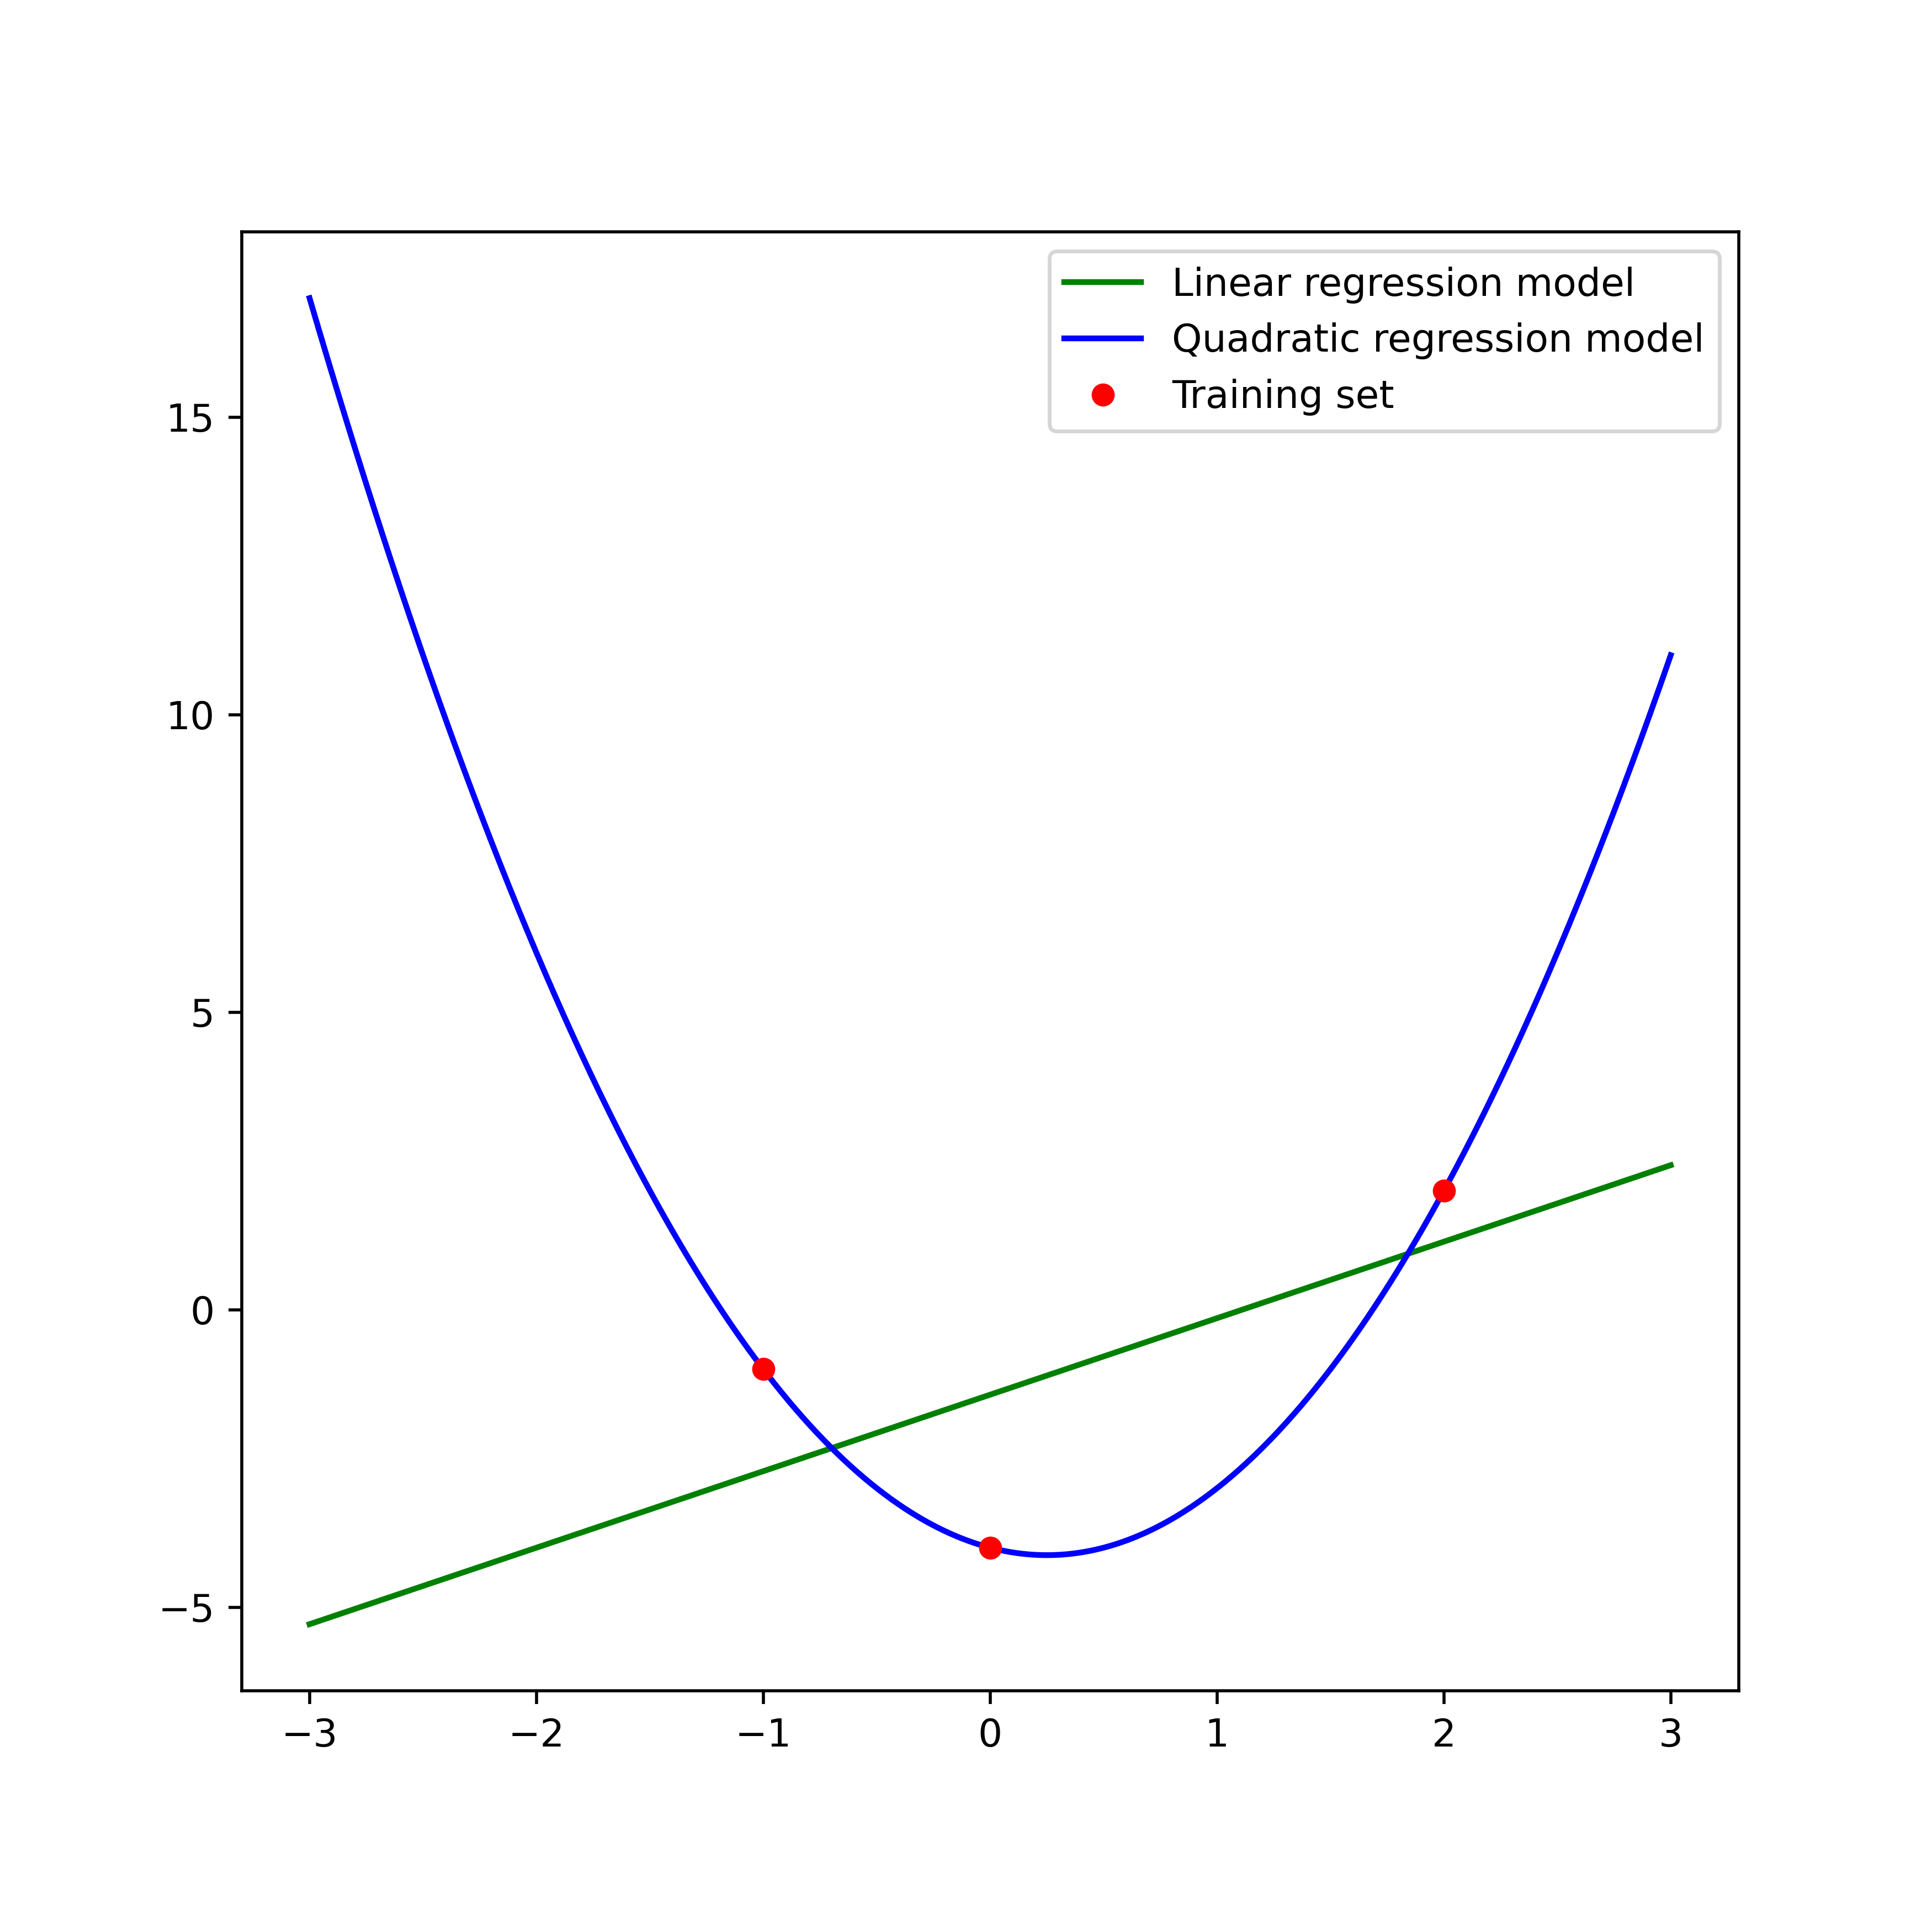
\includegraphics[width=0.5\textwidth]{p01.png}
    \end{center}
\end{enumerate}
\end{homeworkProblem}

\begin{homeworkProblem}
You are given the training data
\begin{equation*}
    \mathcal{T} = \{ (-2, 2)^{\top}, (0, 0)^{\top}, (1, 2)^{\top} \}
\end{equation*}
\begin{enumerate}[a)]
    \item Use the Gaussian kernel with kernel width $\sigma = 1$ and compute by hand the kernel-based model using least squares for the given training data.
    \item Repeat the previous task, but this time you compute by hand the kernel-based model using ridge regression with regularization parameter $\lambda = 1$.
    \item Draw both above models including the training data in one plot.
\end{enumerate}
\end{homeworkProblem}

\begin{homeworkProblem}
Prove Lemma 10.2 from the lecture notes.

Recalling Lemma 10.2:

Let $\{ \boldsymbol x_{i} \}_{i = 1}^{N}$ be a set of points such that $\boldsymbol x_{i} \in \mathbb{R}^{D}$ and let $k: \mathbb{R}^{D} \times \mathbb{R}^{D} \to \mathbb{R}$ be a positive definite kernel. Then, the matrix
\begin{equation*}
    \mathcal{A} = \begin{pmatrix} k(\boldsymbol x_{1}, \boldsymbol x_{1}) & \ldots & k(\boldsymbol x_{1}, \boldsymbol x_{N}) \\
    \vdots & \ddots & \vdots \\
    k(\boldsymbol x_{N}, \boldsymbol x_{1}) & \ldots & k(\boldsymbol x_{N}, \boldsymbol x_{N}) \end{pmatrix}
\end{equation*}

is (symmetric) positive definite.\\

A kernel is a symmetric function. Therefore, the matrix $\mathcal{A}$ is symmetric. The underlying properties of a symmetric matrix are that the eigenvalues are real and the eigenvectors are perpendicular to each other.\\

To prove the positive definite property of the matrix $\mathcal{A}$, the quadratic form can be used. Quadratic form states that if for all $\boldsymbol x != 0$, the product $x^{T} \mathcal{A} x$ is greater than 0, then the matrix is positive definite.\\

We choose to use the orthonormal basis, $\{e_{1}, \ldots, e_{n}\}$, of the eigenvectors corresponding to the eigenvalues, $\{\lambda_{1}, \ldots, \lambda_{n}\}$ of matrix $\mathcal{A}$. We can express any $x$ using the orthonormal basis, $\boldsymbol x = c_{1} e_{2} + \ldots + c_{n} e_{n}$.\\

The quadratic form can then be expressed as:
\begin{equation*}
    \begin{split}
        \boldsymbol x^{T} \mathcal{A} \boldsymbol x & = (c_{1} e_{1}^{T} + \ldots + c_{n} e_{n}^{T}) \mathcal{A} (c_{1} e_{1} + \ldots + c_{n} e_{n}) \\
        & = (c_{1} e_{1}^{T} + \ldots + c_{n} e_{n}^{T}) (c_{1} \mathcal{A} e_{1} + \ldots + c_{n} \mathcal{A} e_{n}) \\
        & = (c_{1} e_{1}^{T} + \ldots + c_{n} e_{n}^{T}) (c_{1} \lambda_{1} e_{1} + \ldots + c_{n} \lambda_{n} e_{n}) \\
        & = c_{1} e_{1}^{T} \cdot c_{1} \lambda_{1} e_{1} + c_{1} e_{1}^{T} \cdot c_{2} \lambda_{2} e_{2} + \ldots c_{n}^{2} \cdot e_{n}^{T} \lambda_{n} e_{n} \\
        & = c_{1}^{2} \lambda_{1} + 0 + \ldots + c_{n}^{2} \lambda_{n} \\
        & = c_{1}^{2} \lambda_{1} + \ldots + c_{n}^{2} \lambda_{n}
    \end{split}
\end{equation*}

\end{homeworkProblem}

\begin{programmingProblem}
In this task, we implement kernel ridge regression. To this end, we start from Example 10.6 from the lecture notes, which is available as Jupyter notebook. However, instead of using scikit-learn to compute the ridge regression model, you replace that part of the code by your implementation of kernel ridge regression, which follows Algorithm 17 from the lecture notes. Due to the existing implementation, it will be easier to evaluate, whether your implementation is correct.
\end{programmingProblem}
\end{document}
